\chapter{Ontwerp}
In dit hoofdstuk wordt het ontwerp van de softwareproducten beschreven.
Tijdens de eerste fase van de afstudeerperiode is er een onderzoek gedaan naar de requirements van het systeem \parencite{DanteOnderzoek}.
Het resultaat van dit onderzoek is een lijst van geprioriteerde requirements en randvoorwaarden waar het systeem aan moet voldoen.
Deze resultaten zijn gebruikt om het softwareproduct te ontwerpen.

\whitespace
Voor het ontwerpen van het systeem is er gebruikgemaakt van een ontwerp framework genaamd het 4 + 1 view model \parencite{4+1ViewModelPaper}.
Het 4 + 1 view model maakt gebruik van 5 verschillende perspectieven om de software inbeeldt te krijgen.
Deze perspectieven zijn scenarios, logical, process, development en physical view (visualisatie is te zien in figuur \ref{fig:4p1Model}).
In de volgende secties worden de perspectieven uitgelegd en ingevuld. 

\whitespace[2]
\begin{graphic}
	\captionsetup{type=figure}
    \caption{4 + 1 Model view model \parencite{4+1ViewModelPaper}}
	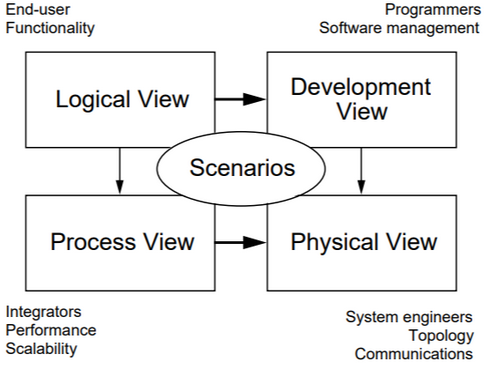
\includegraphics[scale=1.4]{4+1ModelView.png}
	\label{fig:4p1Model}
\end{graphic}

\newpage
\section{Senario's}
Dit worden de Senario's

\newpage
\section{Logical View}
In de volgende sectie wordt de logical view van het 4 + 1 model toegelicht.
Het doel van de logical view is de functionaliteiten van het systeem in beeld te brengen \parencite{4+1ViewModelPaper}.
Dit wordt gedaan door op een abstract niveau naar de structuur en datamodel van het systeem te kijken zonder implementatie details.
De volgende subsecties gaan dieper in op het datamodel en de softwarearchitectuur van het syteem.

\subsection{Datamodel}
Een van de belangrijkste doelen van de afstudeeropdracht is om een nieuw datamodel te maken voor een CMS-systeem.
Dit datamodel moet veel verschillende soorten datastructuren kunnen ondersteunen en deze kunnen presenteren op een klant zijn website.
Het huidige CMS van Snakeware doet dit doormiddel van een complexe structuur.
Deze structuur zorgt ervoor dat het moeilijk is om nieuwe functionaliteit toe te voegen en dat het systeem lastig is te onderhouden.

\whitespace
Daarom heeft het nieuwe datamodel twee belangrijke uitgangspunten om de pijnpunten van het oude CMS te voorkomen.
Het datamodel moet generiek blijven, zodat er veel verschillende datastructuren in opgeslagen kunnen worden.
Door het datamodel generiek en flexibel te houden hoeft het systeem niet uitgebreid te worden om een nieuwe datastructuren te ondersteunen.
Verder moet de structuur van het datamodel simpel blijven zodat het makkelijk te onderhouden is.
Het ontwerp bestaat uit verschillende onderdelen met verschillende taken.
Er wordt op elk onderdeel ingezoomd om een beter beeld te schetsen aan het ontwerp.

\whitespace[2]
\textbf{De content}

\whitespace
Om de content op te slaan wordt er gebruikgemaakt van een geneste structuur.
Om deze geneste structuur op te bouwen is er gekozen om de data op te delen in 2 groepen.

\whitespace
\begin{itemize}
    \item[1] \textbf{Simpele data}: hier worden de basis types van het systeem in opgeslagen.
    Dit zijn de primaire types van de content voorbeelden van deze types zijn tekst, nummer en boolean.
    In het ontwerp is simpele data genoteerd als \textbf{fieldvalues}.
    \item[2] \textbf{Complexe data} is een samenstelling van 0 of meerdere \textbf{fieldvalues}.
    Verder kan complexe data meerdere complexe data bevatten. 
    Hierdoor kunnen er complexe structuren gemaakt worden.
    Dit is gerepresenteerd als \textbf{ItemValues} in het ontwerp.
\end{itemize}

\whitespace
Om structuur aan de data te geven worden ze voorzien door een definitie.
Er zijn definities voor \textbf{itemvalues} en \textbf{fieldvalues}.
Dit is gedaan zodat als er een nieuwe instantie van een stuk complexe data gemaakt moet worden dat dit op basis van de definitie gedaan kan worden.
Om dit weer te geven is er een klassendiagram gemaakt die te zien is in figuur \ref{fig:DeContentClassDiagram}.

\whitespace[2]
\begin{graphic}
    \captionsetup{type=figure}
    \caption{Klassendiagram ItemValue}
    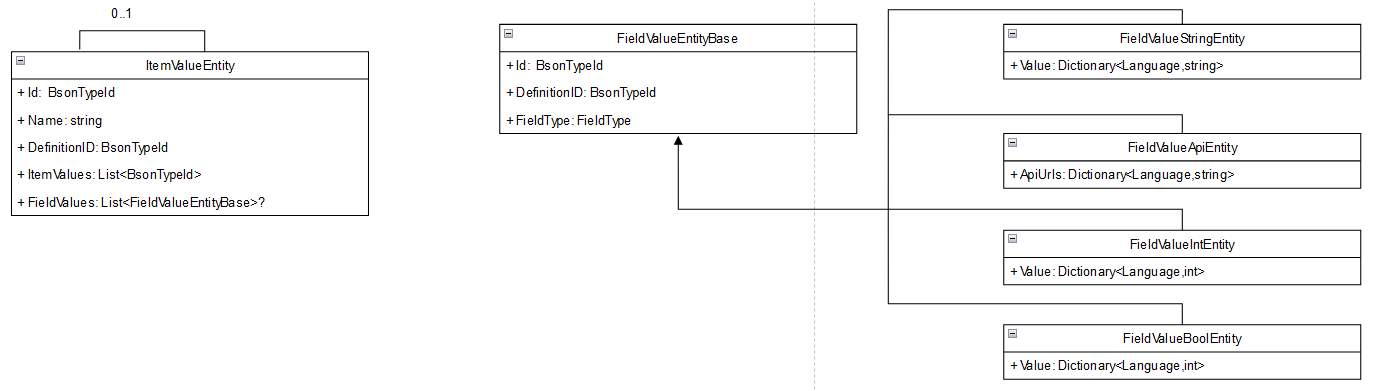
\includegraphics[scale=0.35]{ItemValueEntityClassDiagram.png}
    \label{fig:DeContentClassDiagram}
\end{graphic}

\newpage

\whitespace
\textbf{De componenten}

\whitespace
Om de content een vorm te geven wordt er gebruik gemaakt van componenten.
Voorbeelden van componenten zijn card, artikel en afbeelding.
Door de componenten en de content te scheiden van elkaar geeft dat de mogelijkheid om verschillende componenten te gebruiken op hetzelfde stuk content.
Om ervoor te zorgen dat een component een stuk content kan interperteren wordt er gebruik gemaakt van definities.
Als een stuk content alle \textit{required FiedlDefinitions} heeft kan de component de content renderen.
De componenten worden gerepresenteerd door \textbf{visualcomponent} in het ontwerp. 
Een klasse diagram van de visual component is te zien in figuur \ref{fig:VisualComponentEntityClassDiagram}.

\whitespace[2]
\begin{graphic}
    \captionsetup{type=figure}
    \caption{Klassendiagram VisualComponent}
    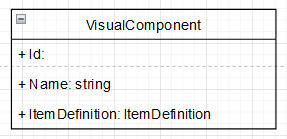
\includegraphics[scale=0.8]{VisualComponentEntityClassDiagram.png}
    \label{fig:VisualComponentEntityClassDiagram}
\end{graphic}

\whitespace
\textbf{De visualalisatie}

\whitespace
Om content op een pagina te renderen moet de content gekoppeld worden samen met de componenten.
Dit wordt gerepresenteerd door het \textbf{itemvisual} in het ontwerp.
Verder kan een itemvisual ook meerdere itemvisuals bevatten waardoor er een geneste structuur ontstaat.
Hierdoor is het mogelijk om complexe websitestructuren te maken.
Verder wordt ook op het itemvisual stijling en layout meegegeven zodat dit niet component afhankelijk is.
Het klassen diagram voor het gehele ontwerp is te zien in figuur \ref{fig:ClassDiagramEntireSystem}

\newpage
\begin{graphic}
    \captionsetup{type=figure}
    \caption{Klassendiagram ItemValue}
    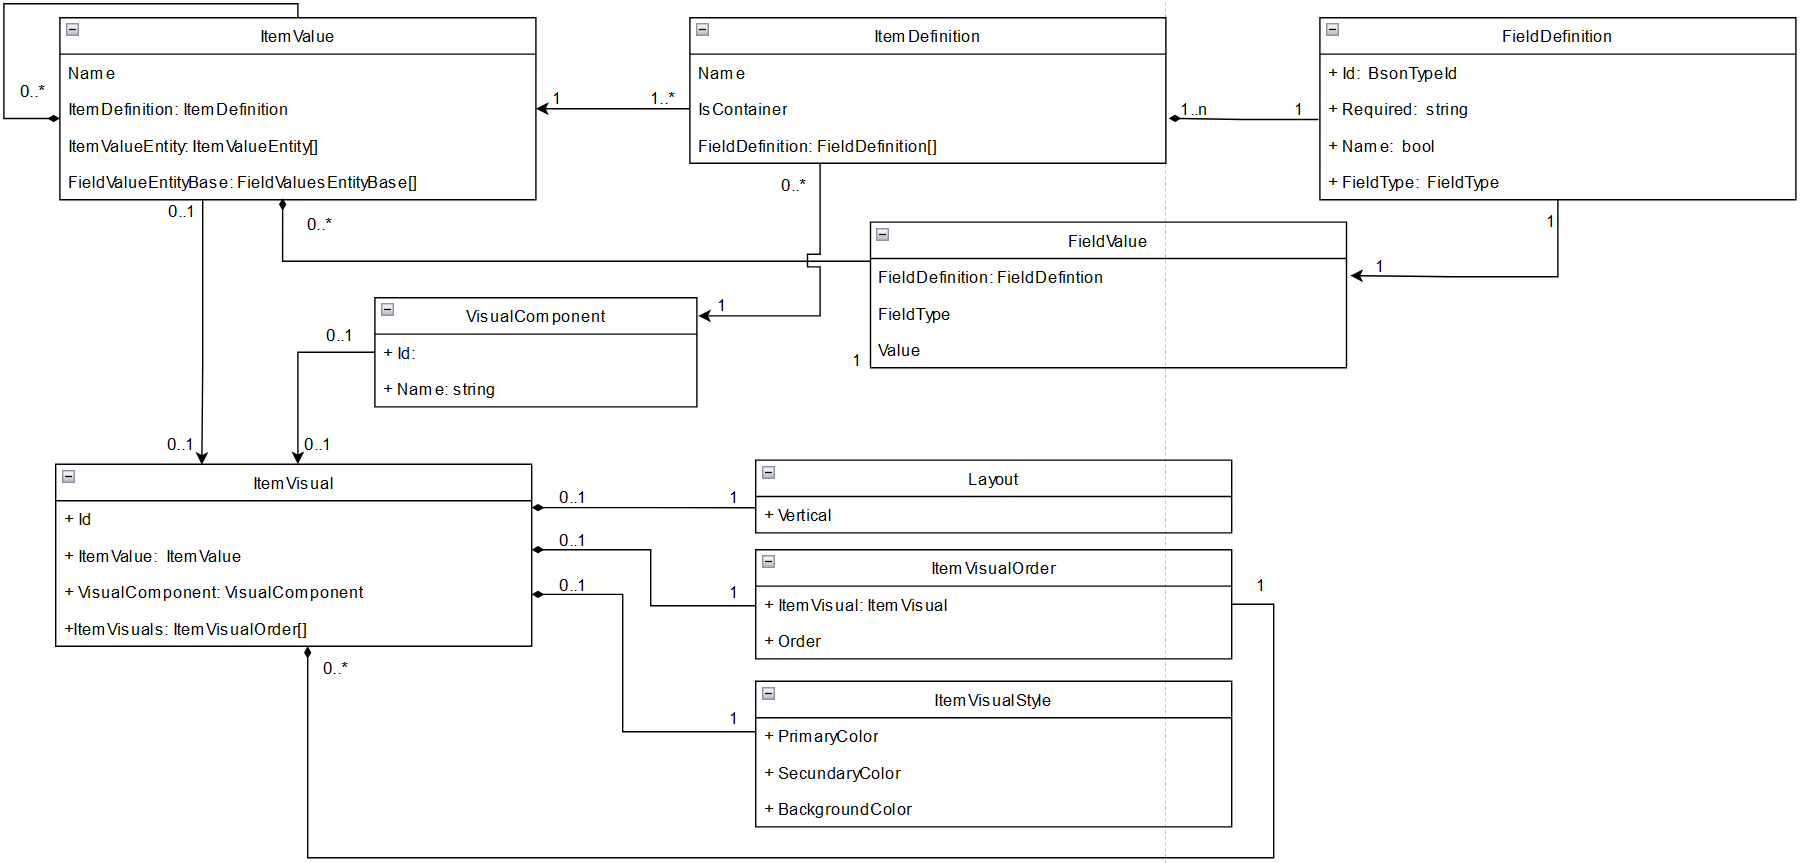
\includegraphics[scale=0.45,angle=90]{ClassDiagramEntireSystem.png}
    \label{fig:ClassDiagramEntireSystem}
\end{graphic}

% \whitespace
% Het datamodel bestaat uit 4 \textbf{objecten} wat in zijn geheel leidt naar de uiteindelijke data die naar de frontend wordt gestuurd.
% Deze objecten zijn Item Definition, Item Value, Visual Component en ItemVisual.
%
% \whitespace[2]
% \textbf{Item value}: De content van het CMS wordt opgeslagen in het itemvalue entiteit.
% Waarbij de waardes van de content worden opgeslagen in een of meerdere \textbf{fieldvalues}.
% Deze fieldvalues kunnen verschillende data types hebben zoals string, boolean en interger.
% Verder kunnen itemvalues meerdere itemvalues bevatten waardoor er complexe datastructuren kunnen ontstaan.
% Om meer inzicht in het datamodel te geven is er een klassendiagram van de itemvalues in figuur \ref{fig:ItemValueEntityClassDiagram}.
%
% \whitespace[2]

%
% \whitespace[2]
% \textbf{Item Definition}: Om structuur aan item values te geven wordt er gebruikgemaakt van een item definition (zie figuur \ref{fig:ItemDefinitionClassDiagram}).
% De belangrijkste functionaliteit van de definition is om aan te geven welke velden er op verschillende items zitten en welke daarvan verplicht zijn.
%
% \whitespace[2]
% \begin{graphic}
%     \captionsetup{type=figure}
%     \caption{Klassendiagram  ItemDefinition}
%     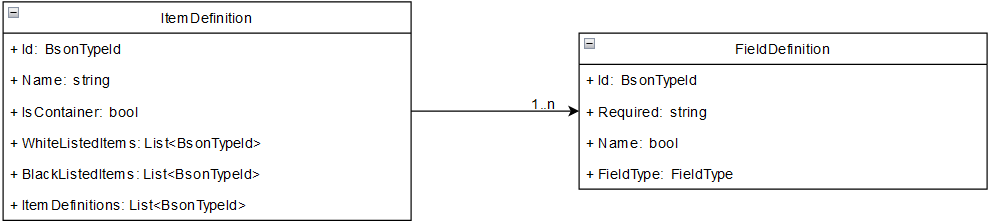
\includegraphics[scale=0.5]{ItemDefinitionClassDiagram.png}
%     \label{fig:ItemDefinitionClassDiagram}
% \end{graphic}
%
% \whitespace
% \textbf{VisualComponent}: Om de data te renderen moeten er componenten gebruikt worden in de frontend om dit af te handelen waar nodig.
% De visualcomponent wordt gebruikt om deze componenten aan te geven welke er zijn en welke definition er bij hoort.
% Een klasse diagram van de visual component is te zien in figuur \ref{fig:VisualComponentEntityClassDiagram}.
%

%
% \whitespace[2]
% \textbf{ItemVisual}: Dit is het object dat de visualcomponent en de item value samen voegt tot een geheel waardoor er content gerenderd kan worden op de pagina.
% Verder geeft dit object ook aan welke mogelijke stijling of layout op het item moet worden toegepast (zie figuur \ref{fig:ItemVisualEntityClassDiagram}.
% Om de data te renderen op een frontend wordt de itemVisual geparesed naar een itemvisualDTO zie figuur \ref{fig:ItemVisualDTOClassDiagram}.
%
% \whitespace[2]
% \begin{graphic}
% 	\captionsetup{type=figure}
% 	\caption{Klassendiagram ItemVisual}
% 	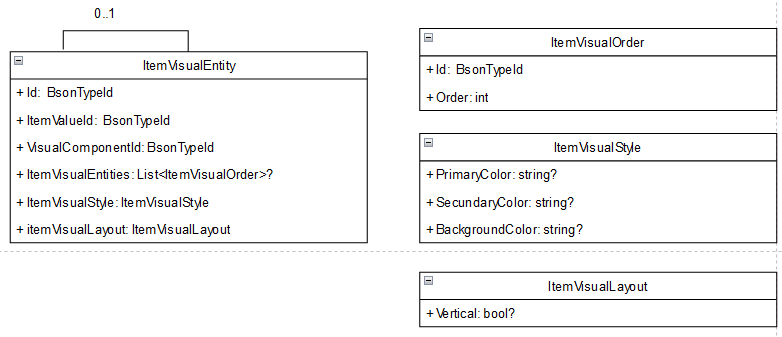
\includegraphics[scale=0.6]{ItemVisualEntityClassDiagram.png}
% 	\label{fig:ItemVisualEntityClassDiagram}
% \end{graphic}
%
% \whitespace[2]
% \begin{graphic}
% 	\captionsetup{type=figure}
% 	\caption{Klassendiagram ItemVisualDTO}
% 	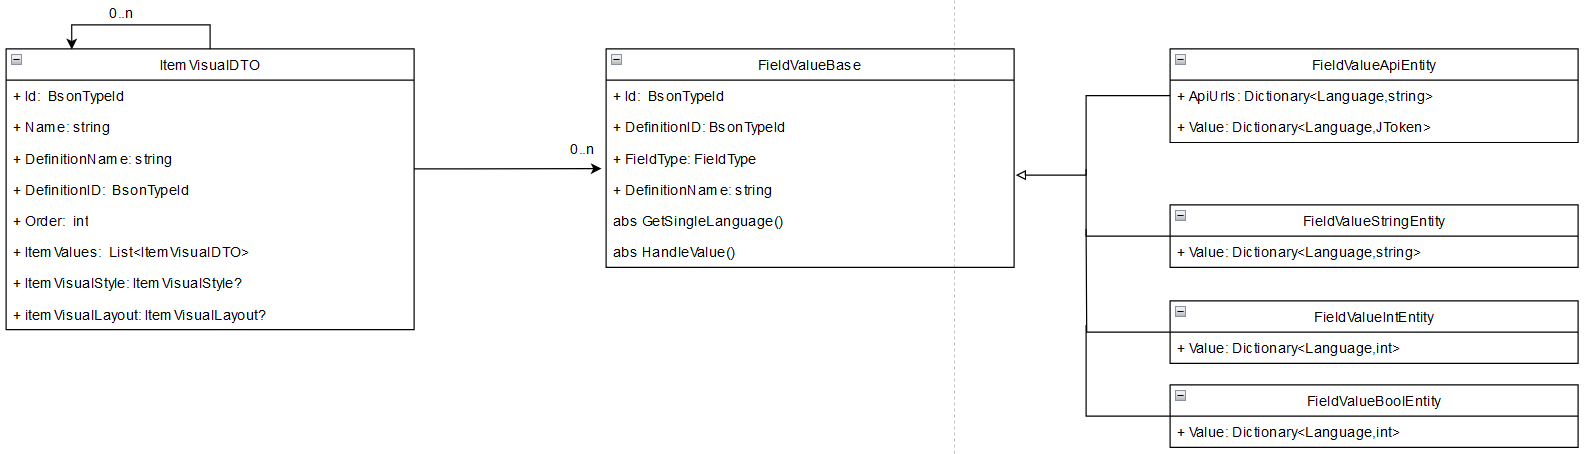
\includegraphics[scale=0.4]{ItemVisualDTO.png}
% 	\label{fig:ItemVisualDTOClassDiagram}
% \end{graphic}

\newpage
\subsection{Software architectuur}
\label{subsecion:SoftwareArhitectuur}
Om in het afstudeerproject niet dezelfde fouten te maken als het huidige \gls{CMS}-systeem is er ook nagedacht over de development principes waar de code aan moet voldoen.
Hiervoor is er gekeken hoe de architectuur zich houdt aan de verschillende SOLID principes \parencite{SOLID}. 
SOLID is een acroniem dat 5 verschillende principes inhoudt.
Deze principes zorgen ervoor dat de code beter te onderhoudbaar is en makkelijker te begrijpen is.
SOLID bestaat uit de volgende principes:

\begin{enumerate}
    \item \textbf{Single-responsibility principle}
    Dit betekent dat een class\slash module, maar 1 verantwoordelijkheid mag hebben.
    Als een class\slash module te veel verantwoordelijkheden heeft dan wordt het moeilijker om de code te begrijpen en aan te passen.

    \item \textbf{Open-closed principle}
    Dit houdt in als class of functie of een andere software entiteit uitgebreid moet worden dat het wordt gedaan door middel van een extensie(open) in plaats van modificatie(closed).
    Hierdoor hou je oude code intact en heb je geen risico dat je bestaande code stuk gaat vanwege de nieuwe functionaliteit die geschreven is. 
        
    \item \textbf{Liskov substitution principle}
    Een class die afgeleid is van een super class zou moeten vervangen kunnen worden van een andere afgeleiden variant van die superclass
    Dit moet gedaan kunnen worden zonder de validiteit (corectness) van het programma te beïnvloeden.
    Door het gebruik van het Liskov substitution principle verhoog je de consistentie en de verwachte uitkomst van het programma.

    \item \textbf{Interface segregation} 
    Een interface moet alleen de methodes geven die nodig zijn voor de client. 
    Geen client moet geforceerd zijn om methodes te implementeren waar die geen gebruik van maakt.
    Dit kan verminderd worden door meerdere kleinere interfaces te maken in plaats van een grote interface.
    Deze interfaces behandelen specifiekere use-cases in plaats van gegeneraliseerde use-cases.
    \item \textbf{Dependency inversion} 
    Een class of module zou niet moeten afhangen van implementaties maar van abstracties.
    Hierdoor de koppelingen van de modules/classes verminderd, en verhoog je de code onder houdbaarheid.
    Om aan dit principe te voldoen wordt er vaak gebruikgemaakt van dependency injection.
\end{enumerate}

\whitespace
Om de verschillende aspecten van SOLID te implementeren is er gekozen om gebruik te maken van handlers.
Hierbij heeft elke handler één taak.
Daarnaast wordt er ook gebruikgemaakt van een repository pattern om met de database te communiceren.
Er is gekozen om gebruik te maken van een repository pattern zodat er geen afhankelijkheid is van de database.
Een sequencediagram van deze architectuur is te zien in figuur \ref{fig:SequenceDiagramHandlerStructure}

\whitespace
\begin{graphic}
    \captionsetup{type=figure}
    \caption{Sequencediagram Handler structuur}
    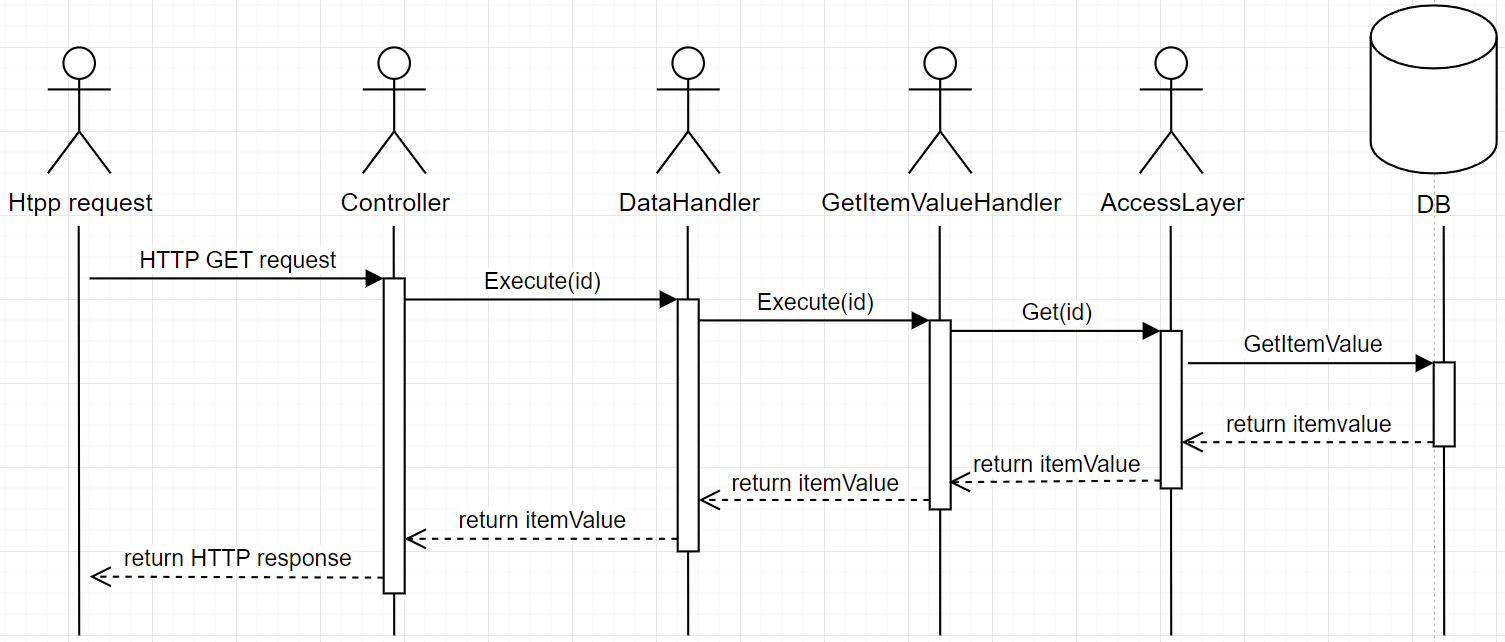
\includegraphics[scale=0.45]{SequenceDiagramArchitectureStructure.png}
    \label{fig:SequenceDiagramHandlerStructure}
\end{graphic}

\whitespace
De verschillende handlers zorgen ervoor dat het single-responsibility principle nagevolgd wordt.
Omdat elke handler maar 1 verantwoordelijk heeft.
Verder worden er kleine interfaces gebruikt om aan het Interface segregation principle te volgen.
En als laatste worden de verschillende dependencies geïnjecteerd (dependency injection pattern) om harde koppeling te voorkomen.


\newpage
\section{Process View}
De process view van het 4 + 1 model dient om het run-time gedrag van het systeem in beeld te brengen \parencite{4+1ViewModelPaper}.
In deze sectie wordt er gekeken hoe het ophalen van de data vanuit de backend werkt.
Verder wordt er ook gekeken hoe de data gerenderd wordt in de frontend.

\subsection{Backend}
Om het proces van het ophalen van de data in beeld te krijgen is er gebruik gemaakt van een sequencediagram.
In figuur \ref{fig:SequenceDiagramItemValueWithChildren} is te zien dat er 4 lagen zijn. 
Dit zijn de Controller, Datahandler, handler en access layer.
De logica om te bepalen of het een succesvolle request was zit in de datahandler.
Logica om het verwachte object terug te krijgen zit in de handler.
En als laatste is er de access layer die de data uit de database haalt.
% Het process begint met een request te maken naar het Get endpoint van de ItemVisualController.
% De datahandler handeld de verschillende responses af voor de request.
% Daarna wordt het GetItemvVisualWithChildren handler voor de itemvisual.
% Het belangrijkste wat deze handler doet is het nesten van de data zodat het uit eindelijk een complete strucuur wordt.
% Daarna wordt er door de itemVisualRepository de data opgehaald uit de database.

\whitespace
\begin{graphic}
    \captionsetup{type=figure}
    \caption{Sequencediagram ItemValue}
    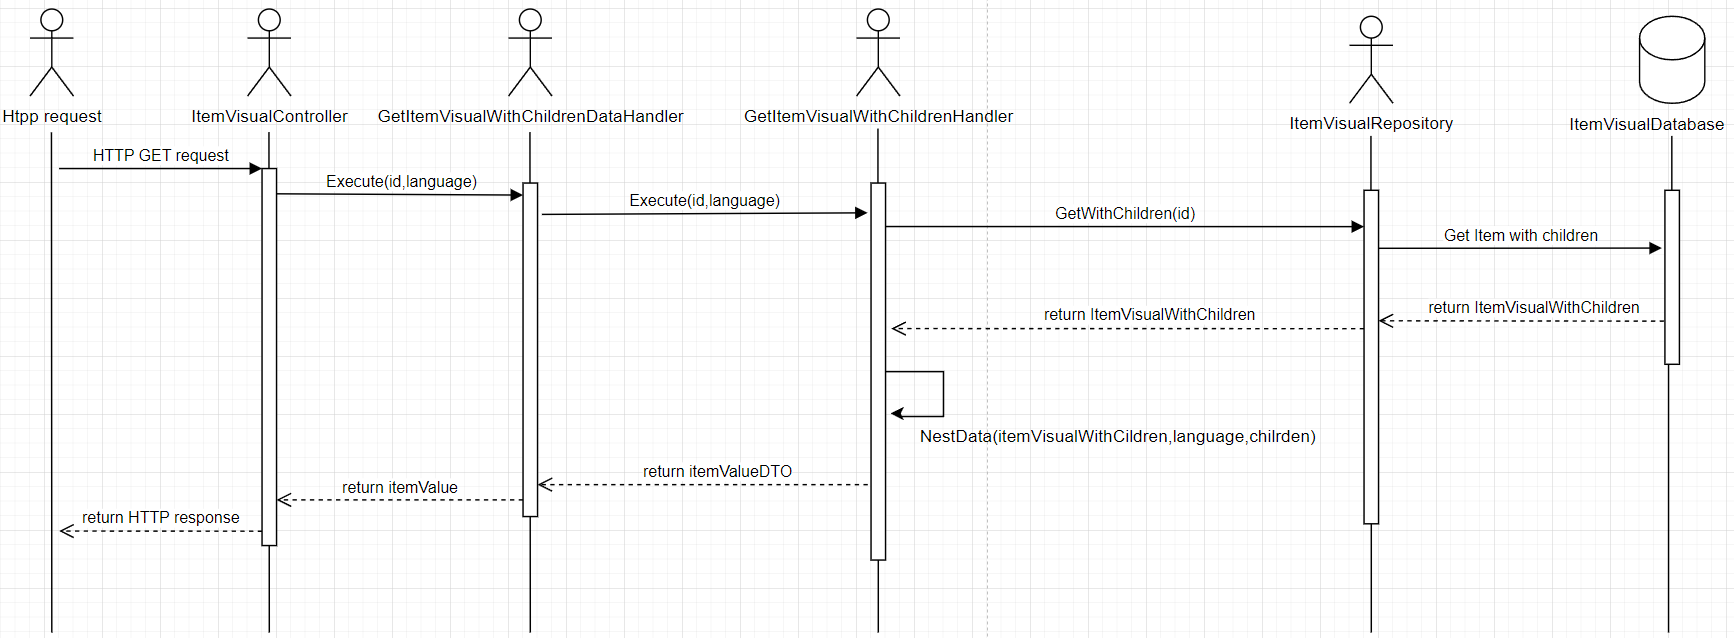
\includegraphics[scale=0.3]{SequenceDiagramItemValueWithChildren.png}
    \label{fig:SequenceDiagramItemValueWithChildren}
\end{graphic}

\whitespace
Een belangrijke functionaliteit in het nesten van de data zodat de frontend het makkelijk kan renderen.
Dit wordt gedaan in de NestData functie om meer inzicht te geven van het proces van de functie is er een flowchart gemaakt (zie figuur \ref{fig:FlowchartNestData}).

\whitespace[2]
\begin{graphic}
    \captionsetup{type=figure}
    \caption{flowchart diagram NestData}
    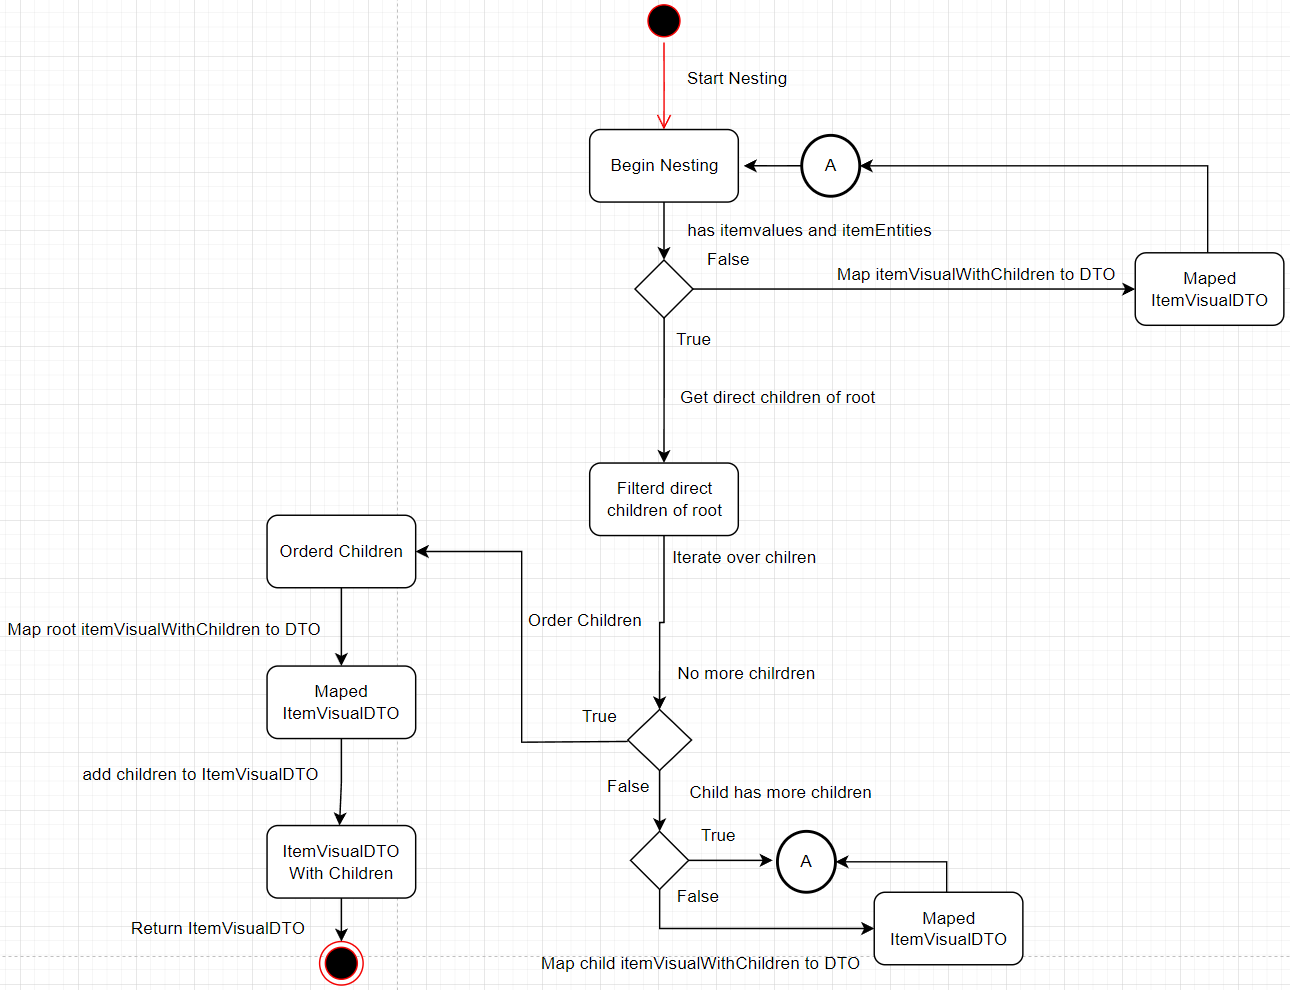
\includegraphics[scale=0.3]{NestingDataFlowchart.png}
    \label{fig:FlowchartNestData}
\end{graphic}

\newpage
\subsection{Frontend}

Om de data te renderen wordt er gebruikgemaakt van 2 verschillende entiteiten types.
Type 1 is een voor gedefinieerd component, hier bij kun je denken aan een artikel, card, afbeelding etc.
Het andere type is een generiek component dat het type 1 componenten encapsuleerd.
Deze componenten worden containers genoemd omdat ze verschillende items encapsuleren.
Verder kunnen containers ook meerdere containers encapsuleren.

\whitespace
\begin{graphic}
    \captionsetup{type=figure}
    \caption{flowchart diagram frontend}
    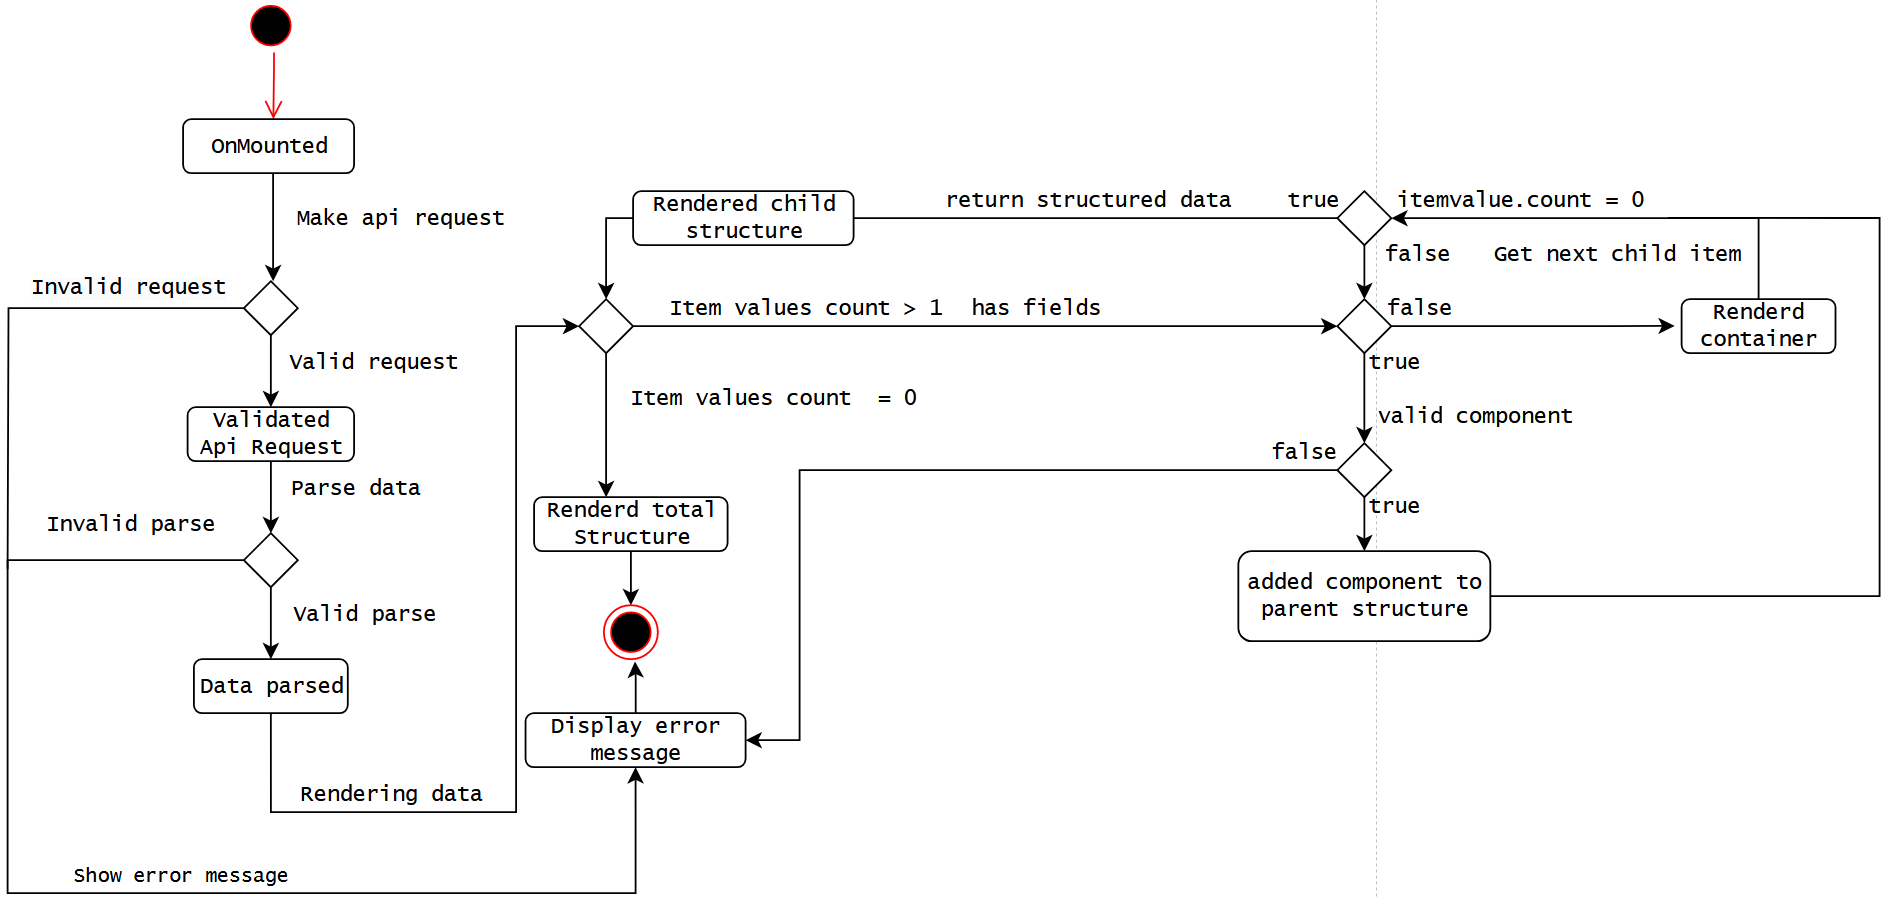
\includegraphics[scale=0.4]{FlowchartFrontend.png}
    \label{fig:FlowchartFrontend}
\end{graphic}

\whitespace
In figuur \ref{fig:FlowchartFrontend} wordt er getoond hoe de frontend met deze container structuur om gaat.
Na het initiële ophalen en valideren van de data begint de main loop van de frontend.
Eerst wordt er gekeken of het huidige object 1 of meer items heeft.
Daarna wordt elk item gerenderd en als het een container is, wordt deze recursief ook gerenderd.
Dit gaat door tot dat alle items gerenderd zijn.


\section{Development view}
De development view is gefocust op het in beeld brengen van de organisatie van software modules \parencite{4p1Model}.
Om dit in beeld te brengen is er gebruikgemaakt van een component diagram.

\whitespace
In figuur \ref{fig:ComponentDiagram} is een component diagram gemaakt.
In het diagram is te zien dat er gebruikgemaakt wordt van een externe authenticatie provider.
Verder is de SOLID implementatie terug te vinden in het diagram (zie \ref{subsecion:SoftwareArhitectuur} voor meer informatie). 
% \todo[inline]{Ik ben het meest onzeker over dit diagram. Want ik heb een gevoel dat ik het veel te erg gegeneraliseerd heb.}

\whitespace[2]
\begin{graphic}
    \captionsetup{type=figure}
    \caption{Deployment diagram van het afstudeerproduct}
    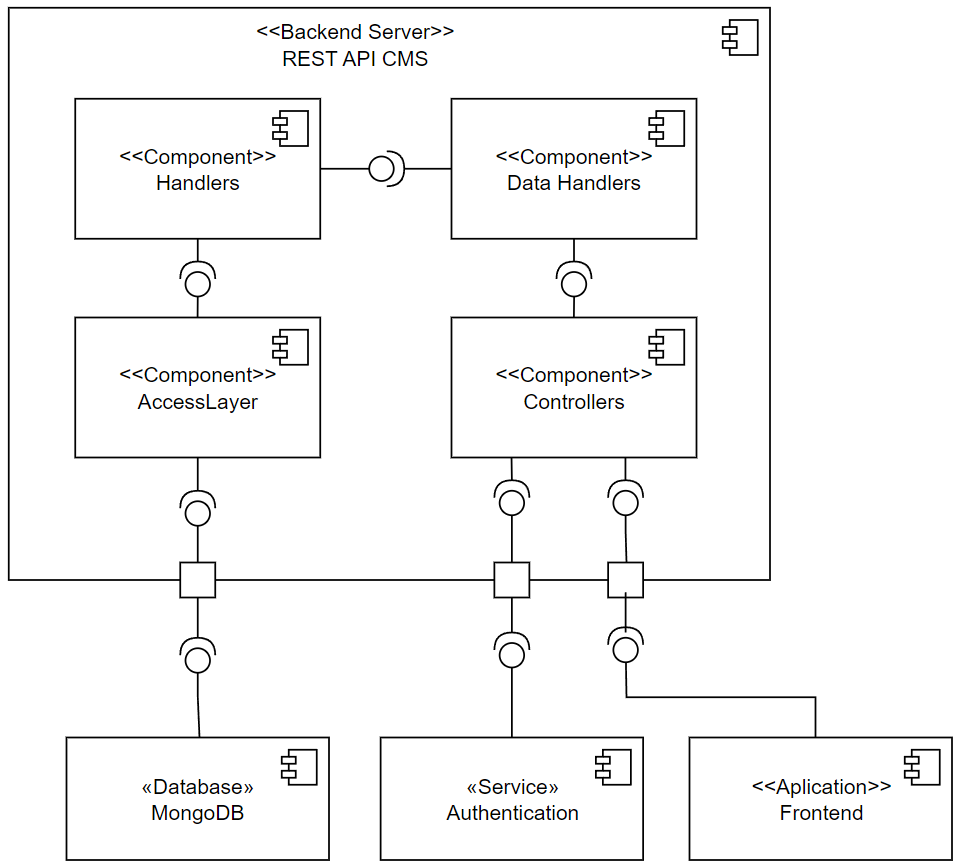
\includegraphics[scale=0.32]{ComponentDiagram.png}
    \label{fig:ComponentDiagram}
\end{graphic}

\section{Physical view}
In de physical view wordt er gekeken naar hoe het systeem gedeployed moet worden en waar.
Om dit in beeld te brengen is er gebruikgemaakt van een deployment diagram \ref{fig:DeploymentDiagram}.
Er is gekozen om gebruik te maken van Docker \Parencite{Docker}.
Docker is een software waarmee software gedeployed kan worden op elke machine op een lichte en efficiente manier \Parencite{Docker}.
Door gebruik te maken van docker kan het systeem gemakkelijk gedeployed worden op cloud hosting platformen en dynamisch schalen.

\whitespace
\begin{graphic}
    \captionsetup{type=figure}
    \caption{Deployment diagram van het afstudeerproduct}
    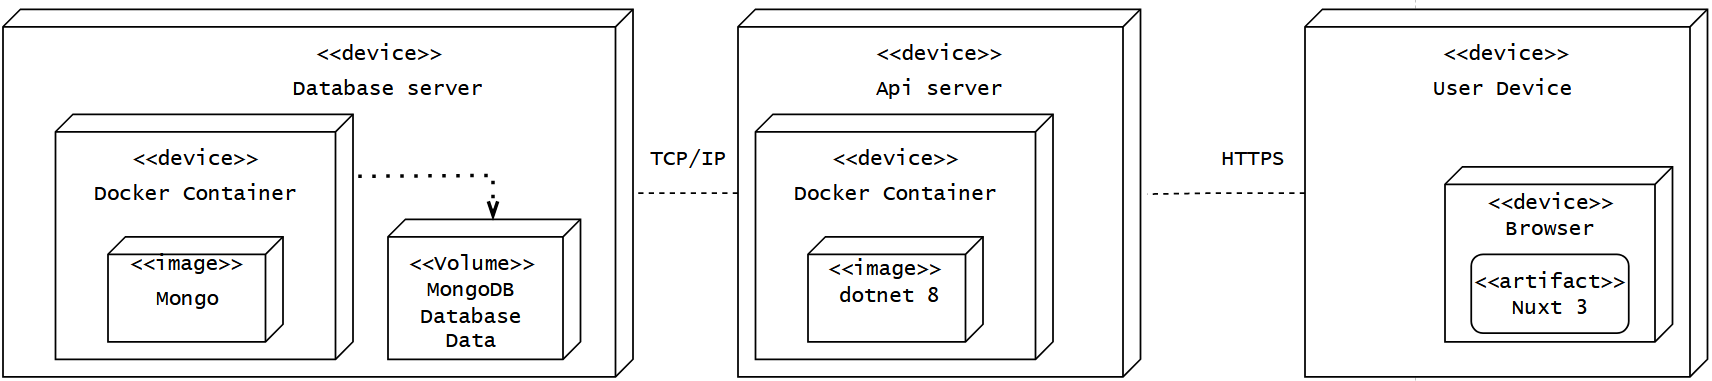
\includegraphics[scale=0.37]{DeploymentDiagram.png}
    \label{fig:DeploymentDiagram}
\end{graphic}


